% Para documento texto corto
%\documentclass[paper=letter,oneside,fontsize=12pt, parskip=full]{article}
\documentclass[paper=letter,oneside,fontsize=11pt, parskip=full]{scrartcl}
%\documentclass{amsart}
%\documentclass[paper=letter,oneside,fontsize=12pt]{scrartcl}

% Establece dimensiones de los margenes
% \usepackage[inner=1.5cm,outer=3cm,top=2cm,bottom=4cm,
% bindingoffset=5mm]{geometry}
\usepackage[left=3cm,right=3cm,top=3cm,bottom=3cm,
bindingoffset=0cm, footskip=0.5cm, headheight=2cm]{geometry}

% Elimina sangrias y aumenta espacio entre parrafos
\usepackage{parskip}

% Permite cambiar margenes derecho e izquierdo
% de secciones de texto con el entorno
% adjustwidth
\usepackage{changepage}

% Permite establecer el espaciado entre lineas
\usepackage{setspace}

% Permite ingresar caracteres acentuados y especiales 
% sin necesidad de emplear comando
% utf8 codificacion de entrada Unicode (mas simbolos que ASCII)
\usepackage[utf8]{inputenc}

% Formato direccione URL
% \usepackage{hyperref}

% T1 encoding for European, English, American text
\usepackage[T1]{fontenc}
% Fuente escalable
\usepackage{lmodern}

% Reemplazo para fuente Arial
% \usepackage{helvet}
% Usa la fuente sans-serif por defecto
% \renewcommand{\familydefault}{\sfdefault}

% Carga babel, idioma ingles
\usepackage[english, spanish]{babel}

% Mejor jsutificacion, tipografia alta calidad.
\usepackage{microtype}
% Para unir columnas y filas en tablas
\usepackage{array}

% Agrega comandos extra al comando tabular
% \toprule, \midrule, \bottomrule
\usepackage{booktabs}
% Tablas con ancho establecido por usuario
\usepackage{tabularx}
% Para posicionamiento preciso de tablas dentro del texto

\usepackage[flushleft]{threeparttable}

\usepackage{float}

% Unir filas en tablas
\usepackage{multirow}

% Permite controlar colores de tablas
\usepackage{xcolor, colortbl}

% Encabezados personalizados
\usepackage{fancyhdr}
\usepackage{graphicx}

% Permite obtener el numero de la ultima pagina
\usepackage{lastpage}

% Paquetes para figuras
% Paquete caption para titulos figuras
% Paquete subcaption para subfiguras
\usepackage{caption}
\usepackage{subcaption}

% Espaciado inteligente
\usepackage{xspace} 

% Para formato de codigo fuente
\usepackage{xcolor}
\usepackage{listings}
% Etiquetas de listandos codigo en españoñ
\renewcommand\lstlistingname{Listado}

\lstset{basicstyle=\ttfamily,
	showstringspaces=false,
	commentstyle=\color{red},
	keywordstyle=\color{blue}}

% Cabeceras
\pagestyle{fancy}
% Borra cabecera y pie actuales
\fancyhead{}
% Cintillo cabecera
%\chead{
%	
\includegraphics[width=150mm]{Imagenes/Cabecera.png}
%}
%\fancyhead[L]{\includegraphics[width=0.3\textwidth]{Imagenes/cabecera.pdf}}
%\fancyfoot[C]{ 
%	\begin{tabularx}{\textwidth}{|m{2.0cm}|X|m{2.5cm}|m{2.0cm}|}
%		\hline			
%			\centering
%			\includegraphics[height=0.8cm]{Imagenes/pie-izq.pdf} &			
%			\centering
%			Confidencial &
%			\centering
%			\includegraphics[height=0.8cm]{Imagenes/pie-der.pdf}  &			
%			\thepage~/~\pageref{LastPage} \\
%		\hline 
%	\end{tabularx}	 
%}

% Comando para formatear y justificar parrafos de código y 
% comandos de shell
% \newcommand{\code}[1]{
%	\begin{adjustwidth}{1.5cm}{0.0cm}
%		\ttfamily
%		#1
%	\end{adjustwidth}}	

% Entorno para formato de secciones de codigo
\newenvironment{code}
	{\begin{adjustwidth}{1.5cm}{0.0cm}\ttfamily}
	{\end{adjustwidth}}

% Entorno para formato de secciones de enlaces
\newenvironment{link}
	{\ttfamily}{}	
	
\definecolor{colorfa}{rgb}{0.3569,0.608,0.8353}
\definecolor{colorfb}{rgb}{0.4392,0.678,0.2784}
\definecolor{colorfc}{rgb}{1.0000,0.361,0.0000}
\definecolor{colorsem}{rgb}{0.1804,0.455,0.7098}
\definecolor{colorfd}{rgb}{0.9294,0.490,0.1922}
\definecolor{colorfe}{rgb}{0.2667,0.329,0.4157}

\newcommand{\fa}{\cellcolor{colorfa}}
\newcommand{\fb}{\cellcolor{colorfb}}
\newcommand{\fc}{\cellcolor{colorfc}}
\newcommand{\sem}{\cellcolor{colorsem}}
\newcommand{\fd}{\cellcolor{colorfd}}
\newcommand{\fe}{\cellcolor{colorfe}}

% Numeracion de paginas
% numeros arabigos
\pagenumbering{arabic}

	\begin{document}
		
		%\title{Informe de Avance de Pasantía}
		%\author{Jose Arias}
		%\address{correo@josearias.com.ve}
		%\date{Septiembre, 2017}
		
		%\maketitle
			
		\begin{titlepage}
		
		\begin{center}		
			
			%\vspace{10cm}
			% 12 puntos = fuente large
			\begin{large}							
				\bfseries
				\uppercase{Universidad Central de Venezuela} \\			
				\uppercase{Facultad de Ingeniería} \\							
				\uppercase{Escuela de Ingeniería Eléctrica} \\
        		\uppercase{Departamento de Electrónica, Computación y Control} \\
        		\uppercase{Anteproyecto de Trabajo Especial de Grado}          	
			\end{large}			
		
			\vfill
			
			\begin{large}
				\bfseries
				\uppercase{Informe de Avance de Pasantía}
			\end{large}
		
			\vspace{2mm}
			
			% 16 puntos = fuente Large de 14 puntos			
			\begin{Large}
				\begin{spacing}{1.2}
					\bfseries				
		      		\uppercase{Diseño de un equipo electrónico controlador de interruptores y atenuadores empleado en la medición de la figura de ruido en dispositivos de radio frecuencia}	
		      	\end{spacing}
			\end{Large}					
			
			\vfill
			
			\begin{flushright}
				Br. Arias Bustamante, Jose A. \\
				C.I. 14.66.744.
			\end{flushright}
		
			\vfill
			
			\begin{center}
				Caracas, septiembre 2017.
			\end{center}
		
		\end{center}
	
	\end{titlepage}
	
	\clearpage
	
	\tableofcontents
		
	\section{Introducción}
		Describe el proceso de instalación adaptador USB/GPIB Agilent 82357B, la instalación y construcción de la librería c de soporte (\texttt{linux-gpib}) a partir del código fuente y la obtención y carga del firmware para el adaptador.
		
	\section{Descripción del Proyecto}
	
	En la figura \ref{Fig:SistemaMedicionFiguraRuido} se muestra un sistema propuesto por Agilent Technologies para medición de la figura de ruido en dispositivos de radio frecuencia y de microondas. Este sistema esta conformado por tres instrumentos fundamentales.
	
	\begin{figure}[!h]
		\begin{center}
			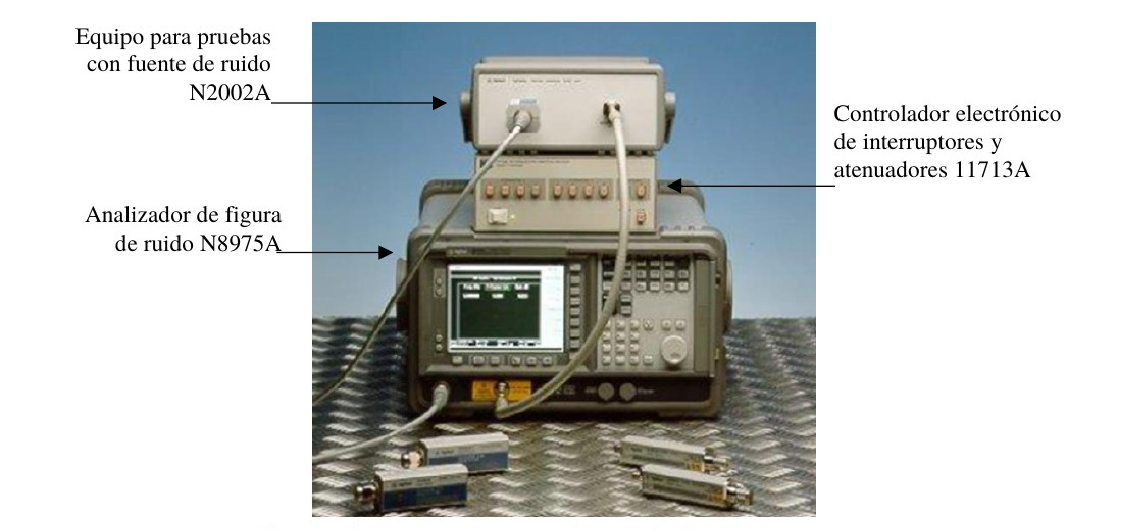
\includegraphics[height=6cm]{Imagenes/SistemaMedicionFiguraRuido.pdf}
			\caption{Sistema para medición de figura de ruido}
			\label{Fig:SistemaMedicionFiguraRuido}
		\end{center}	
	\end{figure}	
	
	\begin{table}[h!]
		\begin{tabular}{p{3cm}l}
			\begin{minipage}{3cm}
				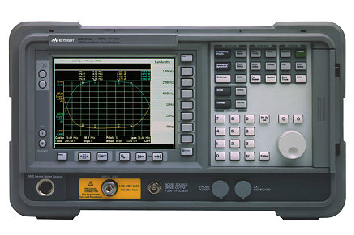
\includegraphics[width=3cm]{Imagenes/N8975A.pdf}
			\end{minipage} &
			Analizador de figura de ruido (NFA) N8975A \\

			\begin{minipage}{3cm}
				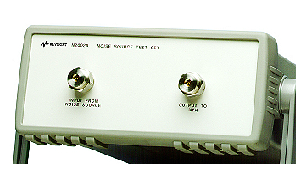
\includegraphics[width=3cm]{Imagenes/N2002A.pdf}
			\end{minipage} &
			Equipo para pruebas con fuente de ruido N2002A \\
			
			\begin{minipage}{3cm}
				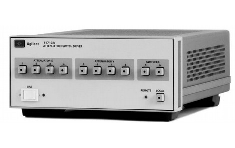
\includegraphics[width=3cm]{Imagenes/11713A.pdf}
			\end{minipage} &			
			Controlador electrónico de interruptores y atenuadores, serie 11713 
		\end{tabular}
	\end{table}

	De los tres equipos listados, el Cendit dispone solo dos de ellos: el analizador de figura de ruido N8975A y el equipo para pruebas con fuente de ruido N2002A. Para que la institución pueda colocar en servicio el SMFR, requiere del controlador electrónico de atenuadores de la serie 11713 de Keysight Technologies. Por motivos presupuestarios, este equipo no ha podido ser adquirido.
	
	Para suplir esta carencia, el Cendit requiere el diseño de un equipo electrónico que pueda suplir la funcionalidad de los equipos de la serie 11713 dentro del sistema. El diseño de este dispositivo es el tema del TEG del cual este documento es un informe de avance de pasantia.
	
	\begin{figure}[!h]
		\begin{center}
			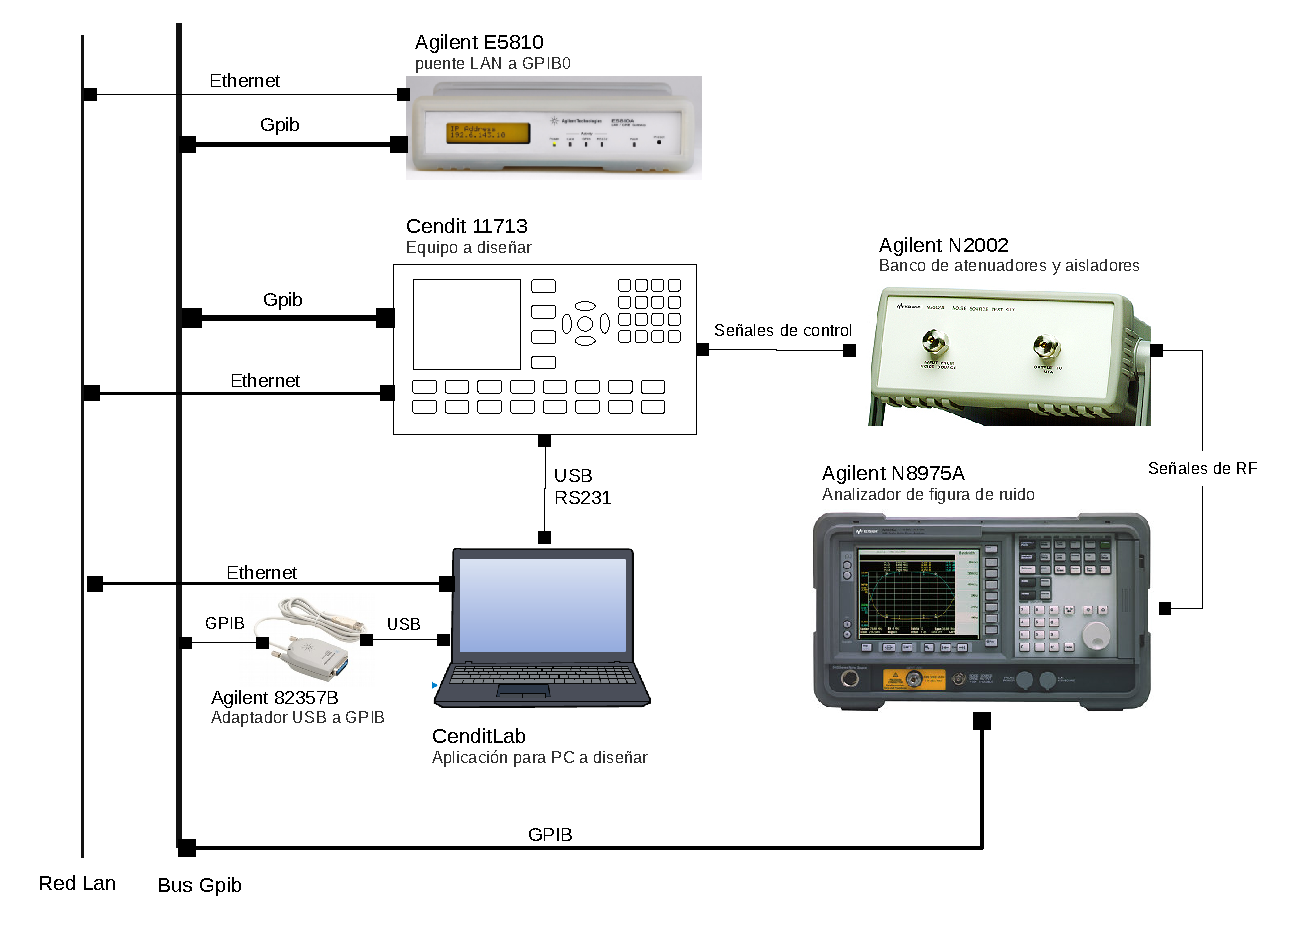
\includegraphics[width=17cm]{Imagenes/DiagramaBloquesSistema.pdf}
			\caption{Esquema de sistema para medición de figura de ruido}
			\label{Fig:SistemaMediciónFiguraRuido}
		\end{center}
	\end{figure}			
	
	


	\begin{figure}[!h]
		\begin{center}
			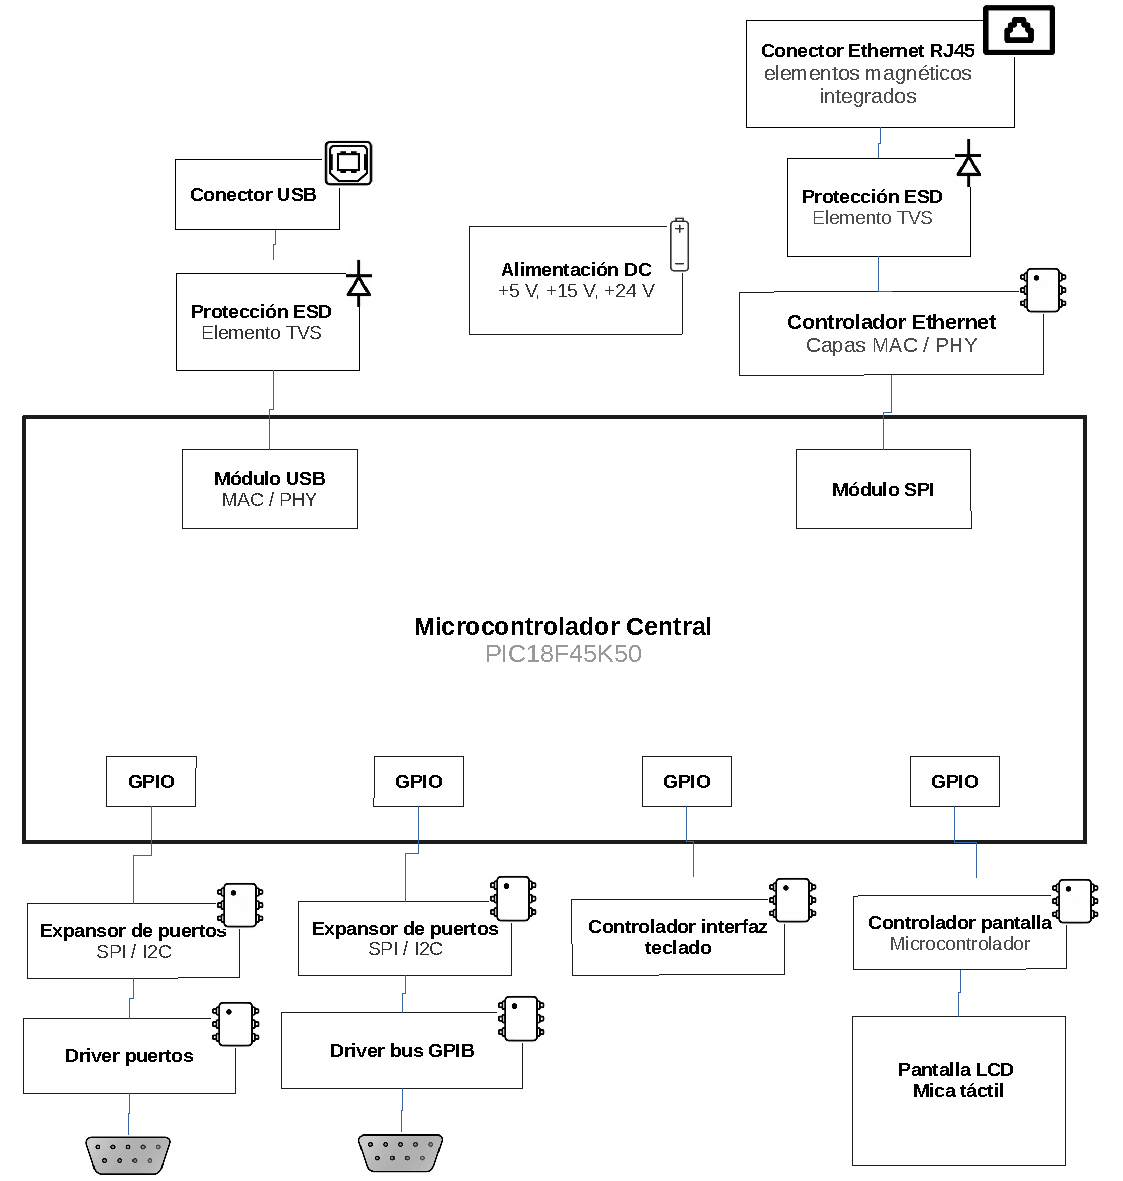
\includegraphics[width=18cm]{Imagenes/DiagramaBloquesHardware2.pdf}
			\caption{Diagrama de Bloques Hardware}
			\label{Fig:Diagrama de Bloques de Hardware}
		\end{center}
	\end{figure}




	\subsection{Metodología Inicial}
	
	\subsection{Cronograma de Actividades}
	
	Al iniciar la pasantía en el Cendit, en el anteproyecto de TEG entregado como parte de los recaudos exigido para su inscripción, se planteo el cronograma de actividades a seguir durante el desarrollo del proyecto que se muestra en la tabla \ref{Tab:CronogramaActividadesInicial}.
	
	\begin{threeparttable}[!h]
		\centering
		\arrayrulecolor{gray}
		\setlength{\extrarowheight}{4pt}		
		\resizebox{\textwidth}{!}{
		\begin{tabular}{|c|l|l|l|l|l|l|l|l|l|l|l|l|l|l|l|l|l|l|l|l|l|l|l|l|l|l|l|l|}
			\hline 			
			\textbf{Semanas} & 1 & 2 & 3 & 4 & 5 & 6 & 7 & 8 & 9 & 10 & 11 & 12 & 13 & 14 & 15 & 16 & 17 & 18 & 19 & 20 & 21 & 22 & 23 & 24 & 25 & 26 & 27 & 28 \\
			\hline
			\textbf{Fase 1}
			& \fa & \fa & \fa & \fa & \fa & \fa & & & & & & & & & & & & & & & & & & & & & & \\			
			\hline			
			\textbf{Fase 2} & & & & & & & \fb & \fb & \fb & \fb & \fb & \fb & \fb & \fb & \fb & \fb & \fb & & & & & & & & & & & \\
			\hline
			\textbf{Fase 3} & & & & & & & & & & & & & & & & & & \fc & \fc & \fc & \fc & \fc & & & & & & \\	
			\hline		
			\textbf{Seminario} & & & & & & & & & & & & & & \sem & & & & & & & & & & & & & & \\
			\hline
			\textbf{Fase 4} & & & & & & & & & & & & & & & & & & & & & & & \fd & \fd & \fd & \fd &  & \\
			\hline
			\textbf{Fase 5} & & & & & & & & & & & & & & & & & & & & & & & & & & & \fe & \fe \\
			\hline	
		\end{tabular}
		}
		\begin{tablenotes}
			\item Fecha de inicio: 6 de Marzo de 2017. 
			\item Jornada de 8 horas diarias, lunes a viernes, de 8:00 AM a 12:00 M y de 1:30 PM a 4:30 PM.
		\end{tablenotes}
		\caption{Cronograma de actividades inicial}			
		\label{Tab:CronogramaActividadesInicial}
	\end{threeparttable}
	
	La ejecución de proyecto se dividió en cinco fases, a desarrollar en un lapso de 28 semanas. A continuación se da una descripción general de las actividades propuestas en cada fase.

	\begin{table}[!h]
		\begin{tabular}{rp{13cm}}
			\textbf{Fase 1} & Preparación e investigación. Dedicada a investigar el funcionamiento de cada uno de los equipos que integran el sistema de medición de figura de ruido. La recopilación y lectura de la documentación de estos equipos que ofrecen las empresas Agilent y Keysight y a través de ensayos sobre el sistema se obtendrá un entendimiento del funcionamiento del mismo. La información obtenida se plasmará en un informe descriptivo del SMFR. \\			
			\textbf{Fase 2} & Diseño de hardware. Comienza con la formulación de un concepto para un equipo que permita suplir la funcionalidad de un equipo de la serie Keysight 11713. Por medio de un proceso iterativo que implica el diseño de hardware, de firmware y mecánico se logrará la documentación de diseño, que permita construir el hardware en la siguiente fase.	\\		
			\textbf{Fase 3} & Implementación del hardware. Se construirá el hardware diseñado y se verificará su desempeño dentro del SMFR. Esta fase implica la depuración firmware y software además de verificar que el hardware cumpla los objetivos de diseño. \\
			\textbf{Fase 4} & Preparación de manuales. Se producirá un manual de usuario para el equipo implementado, que contendrá instrucciones para instalación, operación y resolución de fallas. \\
			\textbf{Fase 5} & Preparación de documentos Cierra el proyecto con la preparación de un informe de pasantía para el Cendit. También se elabora el tomo parra TEG, a presentar en la Escuela de Ingeniería Eléctrica de la UCV.
		\end{tabular}
	\end{table}

	Diversos contratiempos surgidos en los últimos meses han impedido completar algunas de las fases en el tiempo estipulado, provocando que la fases anteriores se traslapen que le prosiguen.
	
	La situación de conflictividad que se presento en la ciudad de Caracas en los últimos meses provocó que el Cendit se viese obligado a recortar la jornada laboral e incluso suspender días completos de actividad en varias ocasiones, para reguardar la integridad física del personal.
	
	Se debe considerar que el proyecto asignado presenta un buen grado de complejidad, 
	abarca el diseño y desarrollo de hardware, software y firmware. En un proyecto complejo, resulta difícil especificar de antemano un plan de trabajo, que detalle con exactitud las actividades a realizar y su extensión en tiempo, antes de involucrarse de lleno en su desarrollo. 
	
	En vista de lo anterior, en este tipo de proyectos, se debe considerar que el cronograma planteado es tentativo, no ha podido ser seguido al pie de la letra, sin embargo ha servido como una guía de la secuencia general de actividades a realizar.

	Las actividades de investigación y desarrollo realizadas para la ejecución del TEG hasta la fecha, han demostrado que el proyecto requiere de tiempo adicional.	

	\section{Actividades Realizadas}
	
	En esta sección se detallan de forma sucinta las actividades realizadas en el desarrollo del TEG, para cada una de las fases, en los últimos 5 meses.
	
	\subsection{Fase 1}
	\subsubsection{Documentación}
	Para entender con propiedad el funcionamiento del SMFR, se debe entender el concepto de figura de ruido. Se realizó un estudio sobre la medición de figura de ruido en dispositivos de RF y microondas, haciendo énfasis en la técnica de medición de figura de ruido conocida como el método del factor Y, la cual es empleada en el SMFR.
	
	Como el sistema mide figura de ruido en dispositivos de alta frecuencia, fue necesario estudiar el concepto de parámetros de dispersión en dispositivos de RF y de microondas. Los parámetros de dispersión son utilizados para caracterizar en frecuencia a dispositivos multipuertos, de forma análoga a las matrices de impedancia o admitancia.
	
	Se recopiló la documentación asociada a los instrumentos y componentes que integran el SMFR. Esta documentación, en forma de manuales de usuario, notas técnicas y hojas de datos, se consiguió de forma libre en internet, en los sitios web de Keysight Technologies y Agilent Technologies. 	
	
	\subsubsection{Investigación y recopilación de software asociado al SMFR}
	
	El proceso de medición en el SMFR puede ser totalmente automatizado por medio de aplicaciones de software apropiadas. El estudio de la documentación del SFMR permitió conocer que existe un buen soporte de software para este sistema, en forma de librerías, entornos de desarrollo y programas de utilidad general.
	
	El estudio de la documentación permitió conocer que existe una especificación que estandariza las comunicaciones entre instrumentos a través de diversos medios de transporte de datos en instrumentos de prueba y medición (Test \& Measurement), como  el bus de interfaz de propósito general (GPIB), o sobre protocolos como TCP/IP o USBTMC empleando puertos estandarizados de PC. Esta especificación se conoce como Virtual Instrument Software Architecture, conocida comúnmente como VISA, es una API que brinda una interfaz uniforme al programador para las operaciones de intercambio de datos. 
	
	Keysight Technologies suministra un amplio soporte de software para los dispositivos del SFMR, en especial un paquete de software conocido como Keysight IO Libraries Suite, que contiene las librerías VISA, exclusivamente para ambiente Windows. 
	
	National Instruments también proporciona librerias VISA para ambiente Windows y para algunas distribuciones de Linux, entre las cuales no se encuentra Ubuntu, 
	sistema operativo que se empleado en el Cendit.
	
	Se realizo un estudio y pruebas con las aplicaciones contenidas en la suite de Keysight, y se empleo la librería VISA que contiene para acceder a los instrumentos del SMFR en ambiente Windows.
	
	Como el Cendit requiere el uso de software libre, se intento instalar las librerías VISA que National Instruments ofrece para Linux, sin resultados satisfactorios, ya que esta empresa proporciona una librería para Ubuntu.	
	
	Ante la carencia de una librería VISA que pueda ejecutarse en Ubuntu, se buscaron alternativas, por ejemplo para el acceso a instrumentos en el bus GPIB se logró por medio de la librería conocida como linux-gpib.
	
	\subsubsection{Informe técnico descriptivo del SMFR}	
	
	\subsection{Fase 2}
	\subsubsection{Diseño de software}
	
	El proyecto requiere de una aplicación de software que permita gestionar y automatizar el proceso de medición con el SMFR empleando un PC. Para lograr un entendimiento de las características que debe poseer una aplicación de tipo T\&M (Test and Measuremt), se estudiaron dos aplicaciones de este tipo que dispone el Cendit.
	
	En particular se estudiaron las aplicaciones EmcTest 32
	
	El estudio se enfoco en dos aspectos fundamentales de estas aplicaciones, como lo son la interfaz de usuario y sus funciones principales. 
	
	Para sistematizar el proceso de captura de requerimientos de software, el tutor sugirió estudiar los estándares ISO/IEC/IEEE, que brindan un marco teorico y una metodología estandarizada para la captura de requerimientos de sistemas de software. Los documentos estudiados se lista a continuación,
	
	\begin{itemize}  
		\item System and Software Engineering Life Cycle Processes Requirements Engineerng (ISO/IEC/IEEE 29148, 2011).
		\item Systems and Software Engineering Vocabulary (ISO/IEC/IEEE 24765, 2011).
		\item Systems and Software Engineering Architecture Description (ISO/IEC/IEEE 42010, 2011).		
	\end{itemize}
	
	Los requerimientos que debe poseer la aplicación
	
	\subsubsection{Documento de captura de requerimientos de software}
	
	\subsubsection{Diseño de hardware}	
	
	Diagrama conceptual y adquisición de componentes.
	
	\subsubsection{Búsqueda, selección y pedido de componentes electrónicos}
	
	\section{Elaboración de instrucciones de trabajo}

	

	

\end{document}